% \textbf{\underline{OZ 5 - Magnetische inductie en de wet van Faraday - Oefening 4:}}
% \vspace{0.5cm}

% Bekijk de drie veldlijnconfiguraties in Figuur 5.4. Welke configuraties zouden bij een magnetisch veld kunnen horen? Bepaal voor die configuratie(s) de objecten die het patroon zouden kunnen creëren (spoel, permanente magneet, stroomvoerende draad, ...).

% \begin{figure}[H]
%     \centering
%     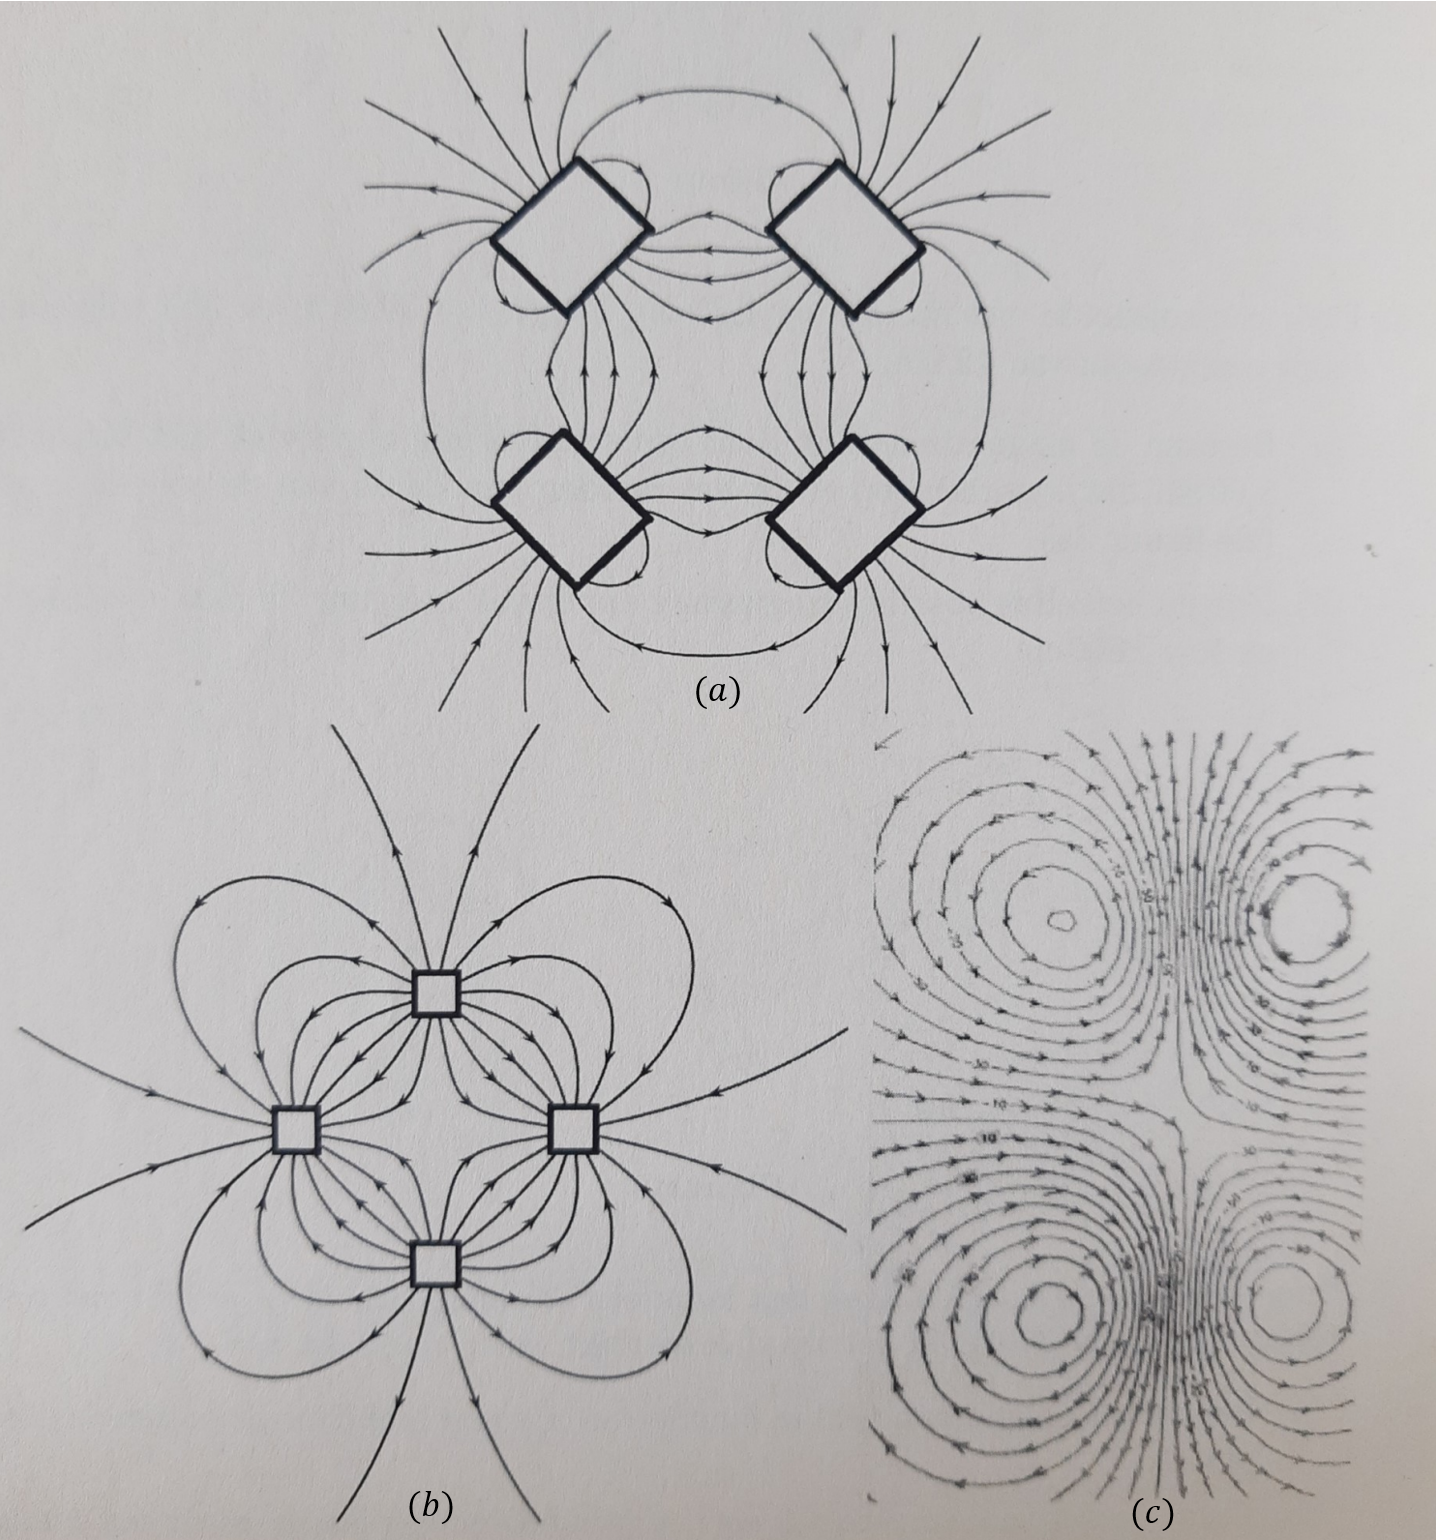
\includegraphics[width=5cm]{oz05/resources/oef-4-opgave.png}
    
%     \textbf{Figuur 5.4}
% \end{figure}

% \begin{enumerate}[(a)]
%     \item De veldlijnen komen langs uit 1 kant van de rechthoeken en komen langs de andere kant terug binnen, dit kan beide een spoel of een permanente magneet voorstellen.
%     \item De veldlijnen komen langs verschillende kanten binnen en buiten, dit is geen magnetisch veld.
%     \item De veldlijnen vormen kringen rond 4 punten, op deze 4 punten kunnen 4 stroomvoerende draden zitten.
% \end{enumerate}

% \vspace{1cm}